\chapter{Parallel Programming}

\section{Motivation for Parallelism}
Power is a critical constraint on the performance of a core executing a single thread.
\begin{center}
    \begin{tabular}{l p{.8\textwidth}}
        \textbf{Dynamic} & Power consumed when signal is changed. \\
        \textbf{Static} & Power consumed to power-up a gate. \\
        \textbf{Static Leakage} & Charge is lost through quantum tunnelling (electrons skip across a gate). This increases exponentially as the gate size is reduced. \\
    \end{tabular}
\end{center}

\begin{definitionbox}{Denard Scaling}
    The dynamic power of a transistor decreases as the size of the transistor decreases.
    \begin{itemize}
        \item Smaller transistors use less power, and can be clocked at higher frequencies.
        \item Smaller transistors also help in increasing the hardware that can be placed on a die of a given size.
    \end{itemize}
\end{definitionbox}

As transistor size has decreased, static leakage has come to dominate power usage, especially at high voltage (required for high clock rate).
\begin{itemize}
    \item Need high voltage to move charge more quickly
    \item Higher voltage $\Rightarrow$ more leakage
    \item Chip must be kept within temperature limits to function
\end{itemize}

Rather than increasing clock rate (becoming very difficult) we can increase the parallelism in the chip \& programs. This is generally much more energy efficient than increasing clock frequency.
\\
\\ There are several ways to mitigate power usage
\begin{center}
    \begin{tabular}{p{.2\textwidth} p{.8\textwidth}}
        \textbf{Clock Gating} & Turn functional units off when unused, deallocate part of the processor (e.g shut down part of the cache), potentially even entire cores (used with arm' big.little architecture) \\
        \textbf{Dynamic Voltage \& Clock} & Reduce performance by adjusting clock rate \& voltage (e.g when battery low). When the processor is not the bottleneck (e.g blottlenecked by screen refresh rate, memory system) there i no need to \textit{'speed ahead'}. This is very popular technique.  \\
        \textbf{Spread Load} & Run many cores at a low clock rate (parallelism). \\
        \textbf{Turbo Boost} & When a single thread is running, can shut off other cores and increase the clock rate temporarily (boost clock rate) on the single core being used. \\
    \end{tabular}
\end{center}

\section{Shared Memory Parallelism}
\subsection{For Loops}
\begin{definitionbox}{OpenMP}
    OpenMP is a specification for language extensions to allow shared-memory parallelism.
    \begin{itemize}
        \item Bindings exist for Fortran, C and C++ (with experimental implementations for Java and C\#)
        \item Allows the programmer to specify how a program should be parallelised
    \end{itemize}
    \begin{minted}{C}
// for example parallelism in for loops
#pragma omp parallel for
for (...) {...}
    \end{minted}
\end{definitionbox}

We can implement for loops in several ways, one is a self-scheduling loop:
\begin{minted}{C}
for (int i=0; i < N ; i++) {
    c[i] = a[i] + b[i]
}
\end{minted}
\begin{minted}{C}
int i;
if (myThreadID() == 0)
    i = 0;

// No thread can cross barrier till all have arrived.
barrier();

for(;;) {
    int local_i = FetchAndAdd(&i);

    if (local_i >= N) 
        break;

    c[local_i] = a[local_i] + b[local_i]
}   

barrier();
\end{minted}
We can perform several optimisations here:
\begin{itemize}
    \item Potentially avoid some barriers (depends on implementation of \mintinline{C}{fetchAndAdd} also)
    \item Work on chunks (if each thread is on a different core, then each has a different L1 cache \& hence having each thread/core work on data with spatial locality is advantageous)
    \item Use cache affinity (previous for loop will have allocated entries in L1 caches of different cores, we can be smart about which cores which threads run on to take advantage of this)
\end{itemize}

\subsection{Atomic Operations}
Using locks is expensive (especially those that use syscalls). hence we can use atomic operations instead.
\begin{itemize}
    \item Many languages provide mechanisms for using atomics (e.g \mintinline{C}{<atomic.h>})
    \item Intrinsics can also be provided on a low level (e.g \mintinline{C}{__sync_fetch_and_add(p, inc)} in C)
    \item The instruction set mut provide some atomic mechanism, in intel this is the \mintinline{asm}{LOCK} prefix, which ensures the operation occurs on a cache line held exclusively (no other cached copies)
    \item In a large system, atomics can cause contention (e.g many fetch \& adds to the same location result in many threads waiting), in a network we can combine these atomic increments(e.g two fetch and increments become a fetch and add 2)
\end{itemize}
OpenMP supports several methods for this:
\begin{minted}{C}
#pragma omp parallel for                                                  \
    default(shared) private(i) All variables except i are shared between  \
                               threads                                    \
                                                                          \
    schedule(static, chunk)    Iterations of the loop can be distributed  \
                               in equal sized blocks to each thread       \
                                                                          \
    reduction(+:result)        Perform a reduction on the variables that  \
                               appear in the argument list (private copy  \
                               created at the end, then all have their    \
                               copies combined)                           
for (i = 0; i < N ; i++)
    result = result + (a[i] * b[i])
\end{minted}

\section{Distributed Memory Parallelism}
\begin{definitionbox}{Mesage Passing Interface (MPI)}
    A standard API for parallel programming using message passing.
    \begin{minted}{C}
MPI_Init       // Initialise MPI 
MPI_Comm_size  // Get the number of processes
MPI_Comm_rank  // Get this process
MPI_Send       // Send a message
MPI_Recv       // Receive a message
MPI_Bcast      // Broadcast data fro the process with rank "root" to all other processes
MPI_Reduce     // Combine values on all processes into a single value using an argument op (e.g sum)
MPI_AllReduce  // MPI_Reduce and broadcast so every process has the reduced value
MPI_Finalize   // Terminate MPI
    \end{minted}
\end{definitionbox}

The key idea with MPI is to use collective operations to write a collection of cooperating processess.
\begin{itemize}
    \item General model to follow is that each process runs the same code (same control flow) and owns a share of the data (Single Program Multiple Data)
\end{itemize}
\begin{sidenotebox}{Stencil}
    A stencil is a program that updates array elements (1d, 2d, 3d +) based on some fixed pattern (the stencil).
    \begin{itemize}
        \item For example Conway's Game of Life uses a stencil to update a cell based on its neighbour's values.
        \item This appears in image processing frequently (e.g blurring, image filtering)
        \item Arises in convolutional neural networks, solving differential equations etc
    \end{itemize}
\end{sidenotebox}
We can demonstrate this with a stencil program.
\subsubsection{With OpenMP}
\begin{minted}{C}
while(!converged) {
    #pragma omp parallel for \
        private(j)           \
        collapse(2)
    for(int j=0; j<M, ++j)
        for(int i=0; i<M, ++i)
            B[i][j] = 0.25 * (A[i-1][j] 
                            + A[i+1][j] 
                            + A[i][j+1] 
                            + A[i][j-1])
    
    #pragma omp parallel for \
        private(j)           \
        collapse(2)
    for(int j=0; j<M, ++j)
        for(int i=0; i<M, ++i)
            A[i][j] = B[i][j]
}
\end{minted}

\subsubsection{With MPI}
The following code is from \href{https://netlib.org/utk/papers/mpi-book/node51.html}{this example} and is written in fortran.
\begin{itemize}
    \item Data is partitioned per process.
    \item Need to consider the \textit{halo} (values just beyond the edges that must be read)
\end{itemize}
\begin{minted}{fortran}
...
REAL, ALLOCATABLE A(:,:), B(:,:)
INTEGER req(4)
INTEGER status(MPI_STATUS_SIZE, 4)
...
! Compute number of processes and myrank
CALL MPI_COMM_SIZE(comm, p, ierr)
CALL MPI_COMM_RANK(comm, myrank, ierr)

! compute size of local block
m = n/p
IF (myrank.LT.(n-p*m)) THEN
    m = m+1
END IF

! Compute neighbors
IF (myrank.EQ.0) THEN
    left = MPI_PROC_NULL
ELSE
    left = myrank - 1
END IF
IF (myrank.EQ.p-1)THEN
    right = MPI_PROC_NULL
ELSE
    right = myrank+1
END IF

! Allocate local arrays
ALLOCATE (A(0:n+1,0:m+1), B(n,m))
...
! Main Loop
DO WHILE(.NOT.converged)
    ! compute
    DO i=1, n
        B(i,1)=0.25*(A(i-1,j)+A(i+1,j)+A(i,0)+A(i,2))
        B(i,m)=0.25*(A(i-1,m)+A(i+1,m)+A(i,m-1)+A(i,m+1))
    END DO

    ! Communicate
    CALL MPI_ISEND(B(1,1),   n, MPI_REAL, left,  tag, comm, req(1), ierr)
    CALL MPI_ISEND(B(1,m),   n, MPI_REAL, right, tag, comm, req(2), ierr)
    CALL MPI_IRECV(A(1,0),   n, MPI_REAL, left,  tag, comm, req(3), ierr)
    CALL MPI_IRECV(A(1,m+1), n, MPI_REAL, right, tag, comm, req(4), ierr)

    ! Compute interior
    DO j=2, m-1
        DO i=1, n
            B(i,j)=0.25*(A(i-1,j)+A(i+1,j)+A(i,j-1)+A(i,j+1))
        END DO
    END DO
    DO j=1, m
        DO i=1, n
            A(i,j) = B(i,j)
        END DO
    END DO

    ! Complete communication
    DO i=1, 4
        CALL MPI_WAIT(req(i), status(1.i), ierr)
    END DO
...
END DO
\end{minted}

\section{Snooping Cache Coherency Protocols}
\begin{center}
    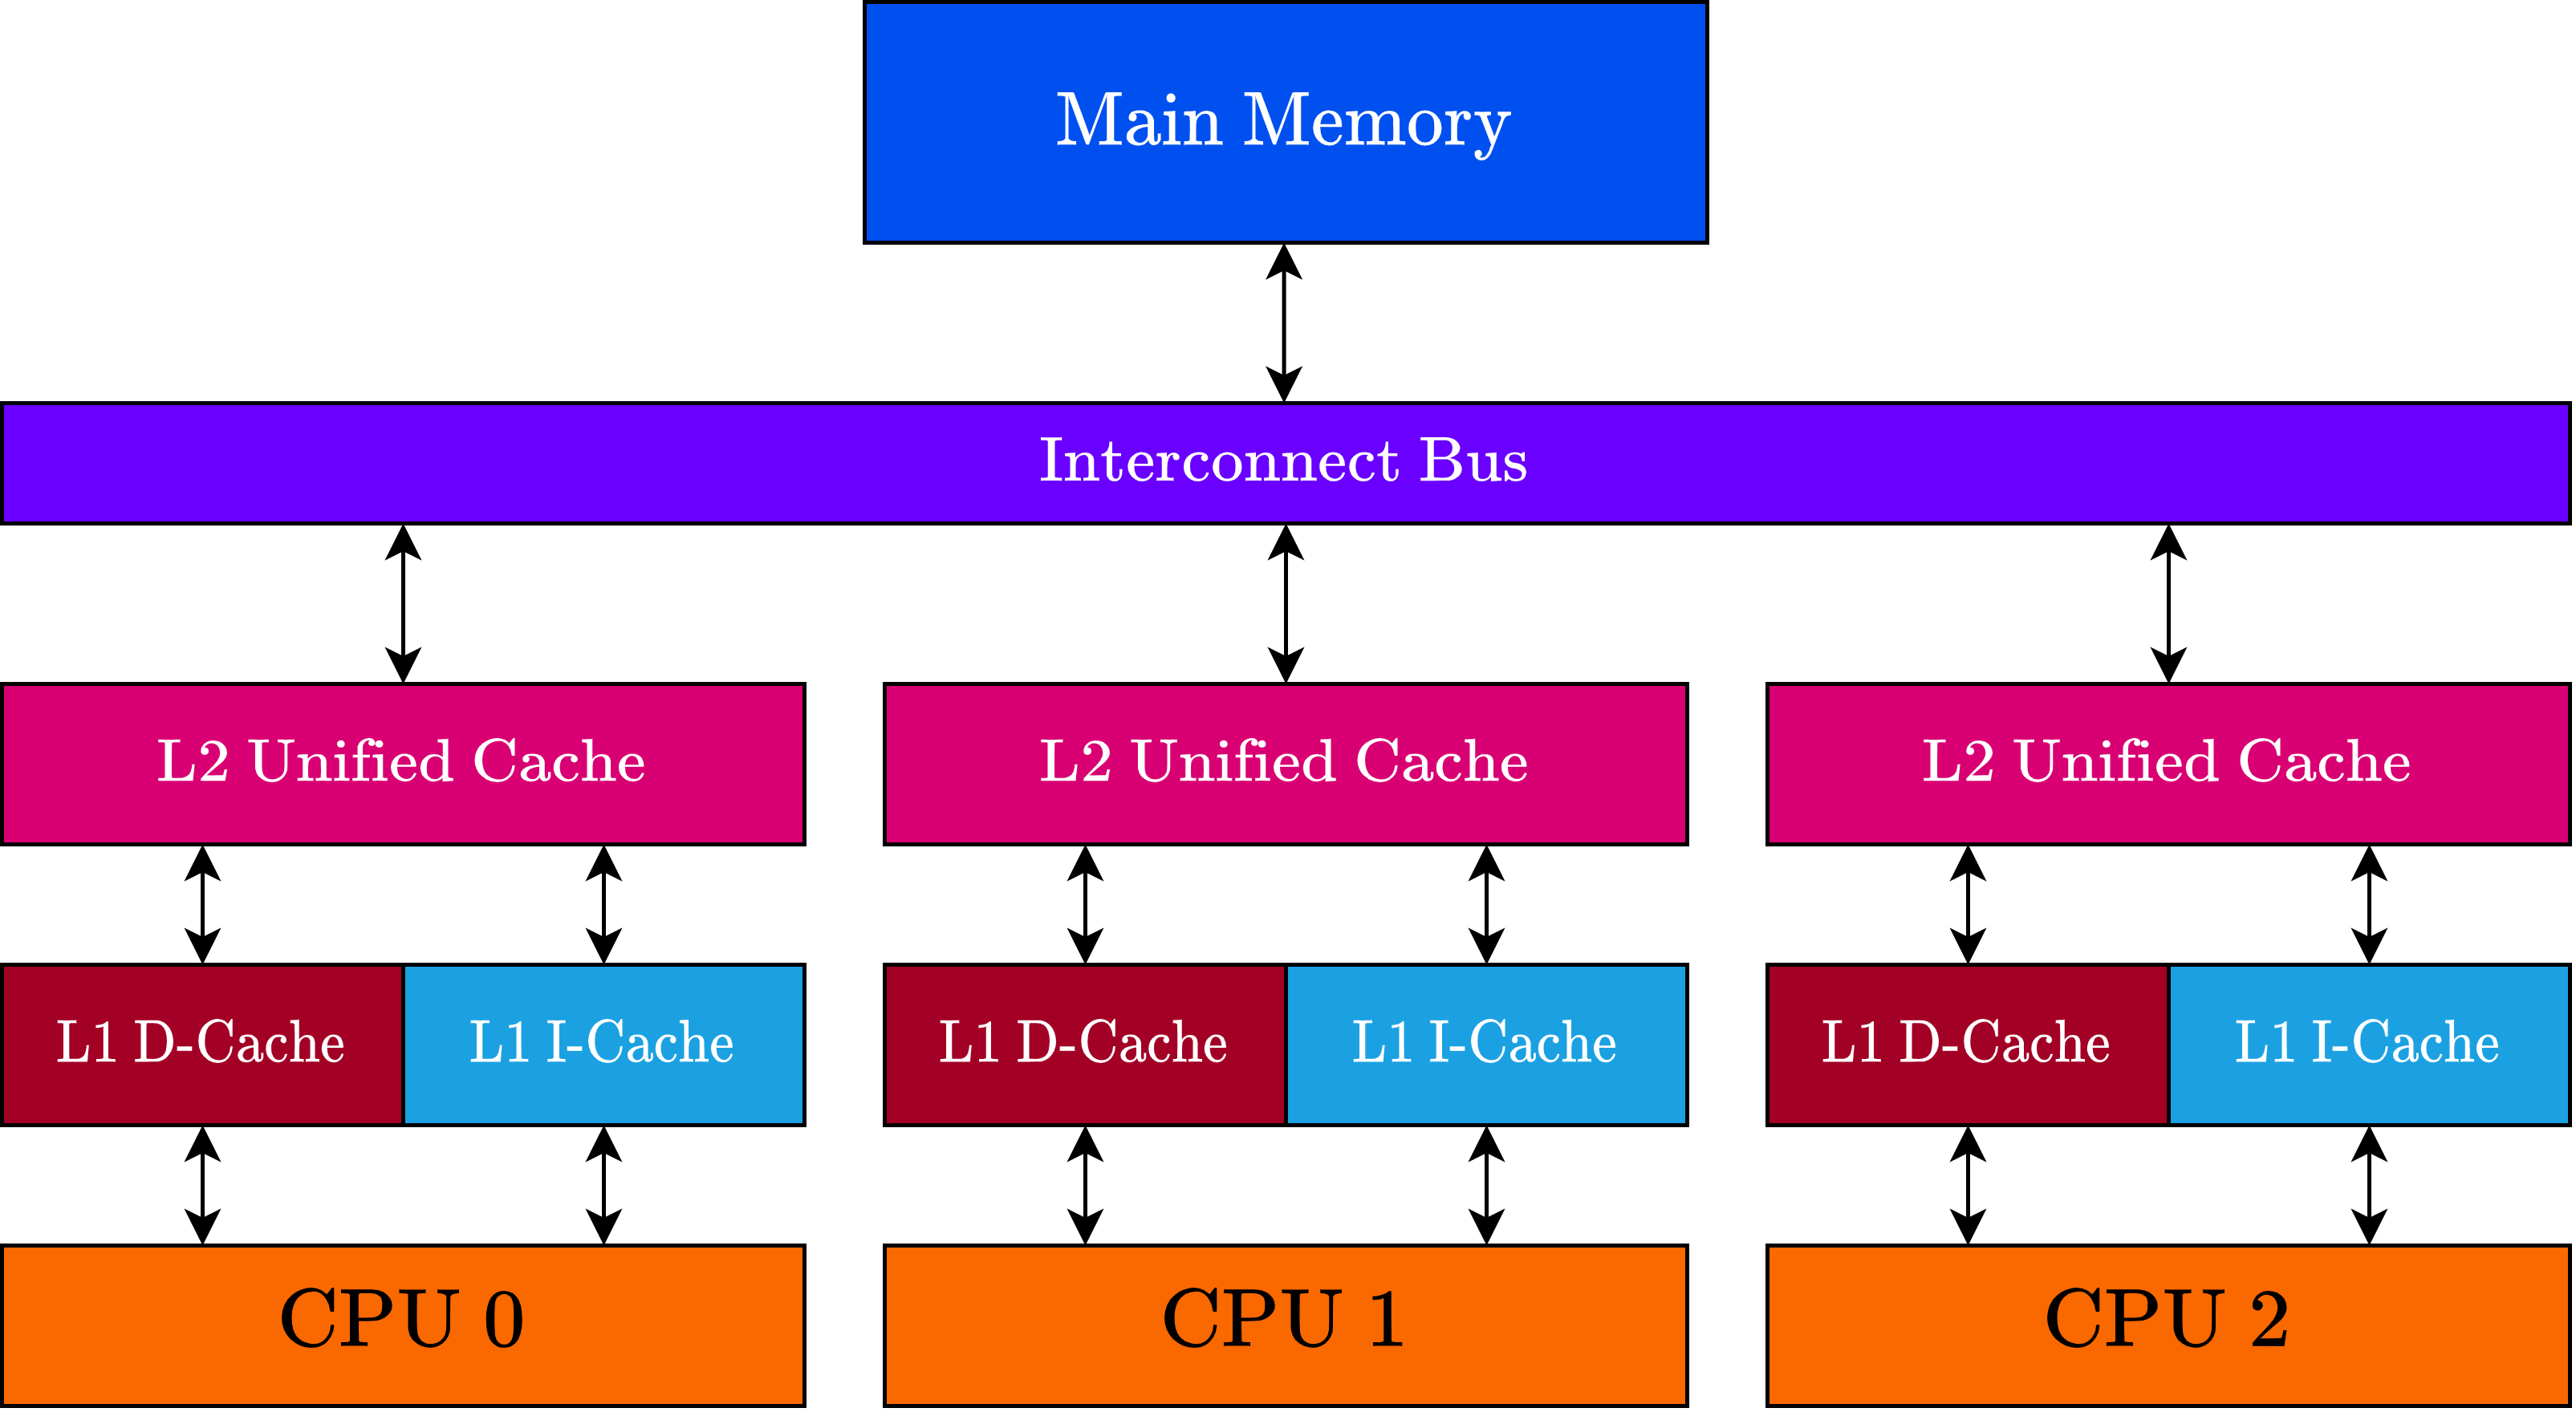
\includegraphics[width=.8\textwidth]{parallel_programming/images/basic_cache_hierarchy.drawio.png}
\end{center}
Given a value can be in multiple caches, at multiple levels
\begin{itemize}
    \item Which is the latest version of the cache line?
    \item Which parts of the line are actually outdated?
    \item Can the cached copy be used?
\end{itemize}
The goal is to ensure the result of any execution is the same as if operations in each thread were executed in a sequential order (sequential consistency), or something weaker but with enough guarantees to allow concurrent programs to be written correctly.
\begin{sidenotebox}{Sequential Consistency Never!}
    sequential consistency is a very strong memory model, and is not typically implemented by any architectures.
\end{sidenotebox}

\subsection{Invalidation}
Instead of updating values in all caches on a write, we instead invalidate.
\begin{itemize}
    \item On the first write, send invalidation signal to other core's cache controllers.
    \item Hence after first write, we know we have the \textit{only} copy, so no need to communicate further writes.
    \item Sharing state stored in extra bits added to the cache line.
\end{itemize}
This is typically faster than updating other cache entires on write, unless the data is usually required immediately.
\\
\\ A \textit{snooping cache controller} is placed between the L2 cache and the interconnect bus to monitor for invalidations, and send invalidations.

\subsection{Berkely Protocol}
Each cache line contains a state:
\begin{center}
    \begin{tabular}{l p{.8\textwidth}}
        \textbf{Invalid} \\
        \textbf{Valid} & Clean, potentially shared \& unowned \\
        \textbf{Shared-dirty} & modified, possibly shared, owned \\
        \textbf{Dirty} & modified, not aliased/only copy, owned \\
    \end{tabular}
\end{center}

On a read hit, a \textbf{clean} or \textbf{dirty} entry can be read (read from the owner), \textbf{invalid} requires an access on the interconnect bus and \textbf{shared-dirty} requires an invalidation to be sent.

\subsubsection{Read Miss}
\begin{minipage}{.5\textwidth}
    \begin{minted}{Python}
Broadcast the request on the interconnect bus

if other cache has line as DIRTY or SHARED-DIRTY:
    get the cache line
    set its cache line to SHARED-DIRTY
    set our cache line to VALID
else:
    load line from main memory
    set our cache line to VALID
    \end{minted}
\end{minipage}
\begin{minipage}{.5\textwidth}
    \subsubsection{Write Hit}
    \begin{minted}{Python}
if cache line is VALID or SHARED-DIRTY:
    send invalidation to interconnect bus
    set our cache line to DIRTY
    \end{minted}
    
    \subsubsection{Write Miss}
    \begin{minted}{Python}
get line from owner
set all copies of the line to INVALID
set our cache line to DIRTY
    \end{minted}
\end{minipage}
\begin{center}
    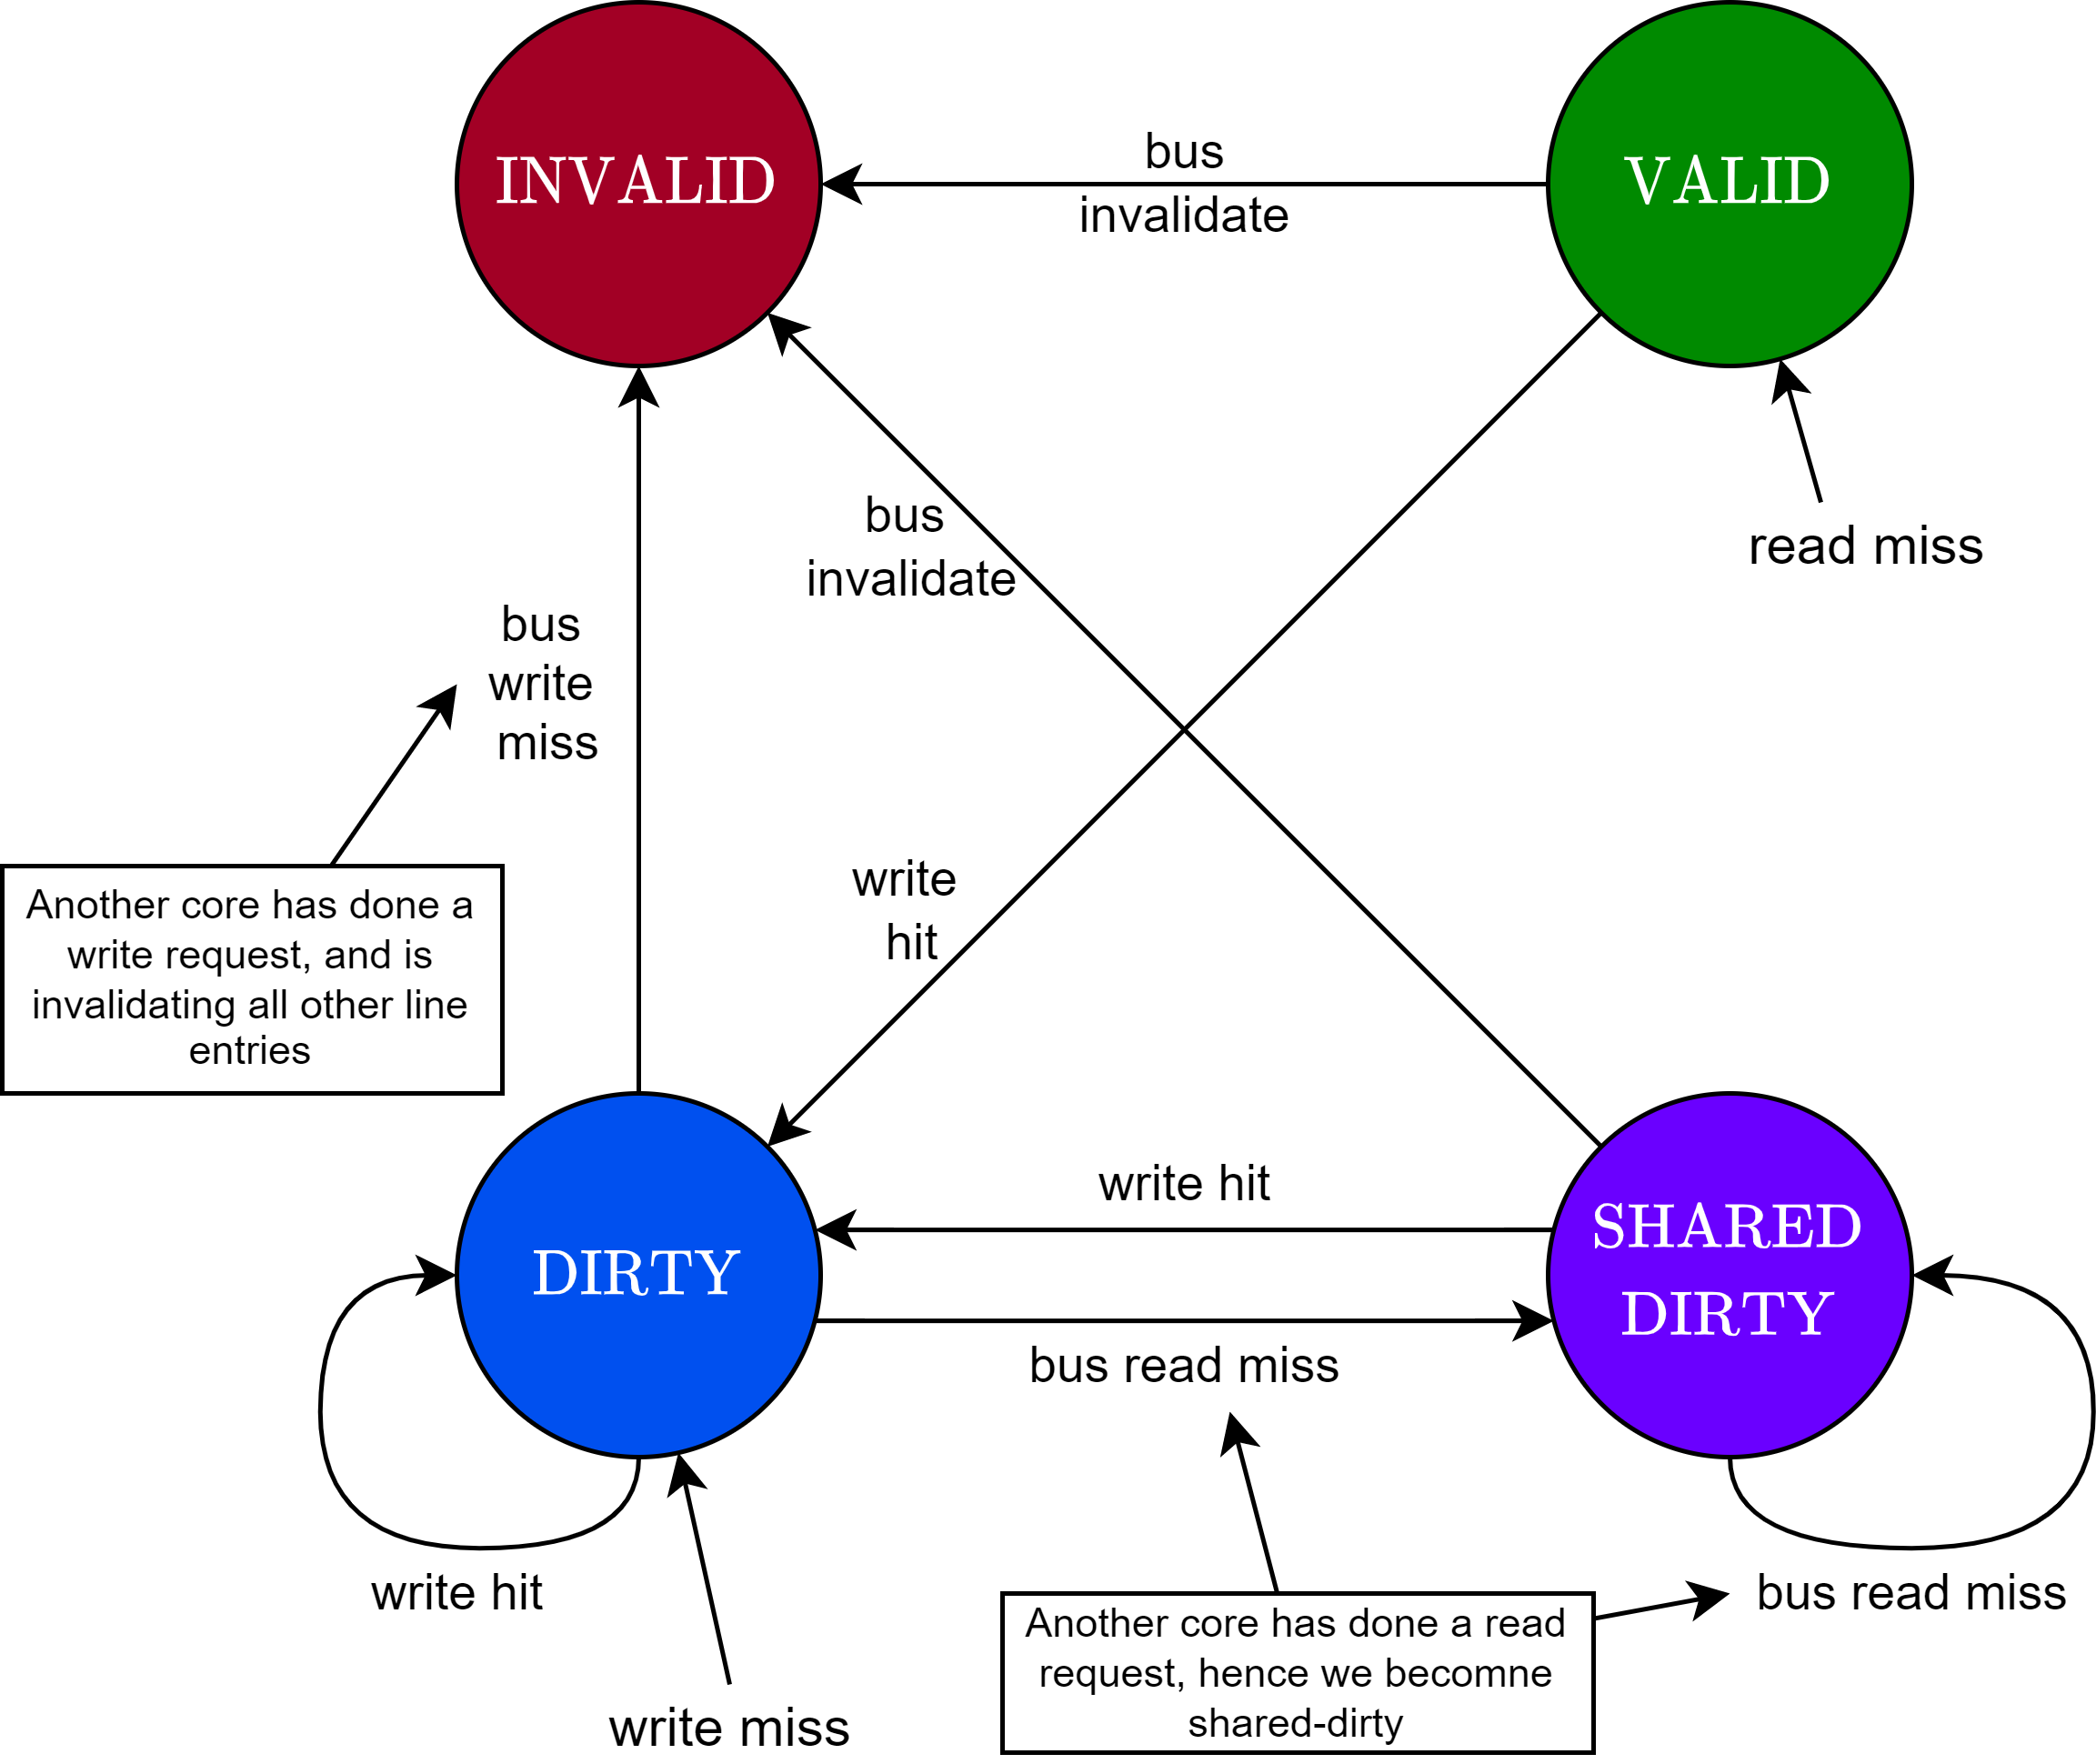
\includegraphics[width=.7\textwidth]{parallel_programming/images/berkley_transitions.drawio.png}
\end{center}
There are alternatives ssuch as:
\begin{center}
    \begin{tabular}{l p{.8\textwidth}}
        \textbf{MESI Protocol} & Clean for exclusive state (no miss for private data on write) \\
        \textbf{Illinois Protocol} & Cache supplies data when shared state (no memory access) \\
    \end{tabular}
\end{center}
The bus and CPU may contend for cache access:
\begin{itemize}
    \item Can duplicate the tags of the L1 cache to allow CPU and snooping cache controller to check in parallel.
    \item Can use the L2 cache as a filer (L2 contains all of L2 - \textit{multi-level inclusion}), hence bus can check L2 cache, if not present then a lien is also not present in L1.
    \item Creates constraints on the cache design.
\end{itemize}

\section{Synchronisation}
\unfinished

\section{Scalable Shared Memory}
\unfinished